\documentclass{article} % Tạo một bản báo cáo
\usepackage[utf8]{vietnam}
%\usepackage[utf8]{inputenc} 
%\usepackage[T5]{fontenc} % Để sử dụng Tiếng Việt 
\usepackage[fontsize=13pt]{scrextend} % Set fontsize=13pt
\usepackage[paperheight=29.7cm,paperwidth=21cm,right=2cm,left=3cm,top=2cm,bottom=2.5cm]{geometry} % Chuẩn A4, căn lề phải, trái, trên, dưới.
\usepackage{mathptmx} % Time New Roman
\usepackage{graphicx} % Thư viện chèn ảnh
\usepackage{float} % Set vị trì chèn ảnh 
\usepackage{tikz} % Thư viện tạo khung bìa 
\usetikzlibrary{calc} % Thư viện tikz
\begin{document}
\begin{titlepage}
    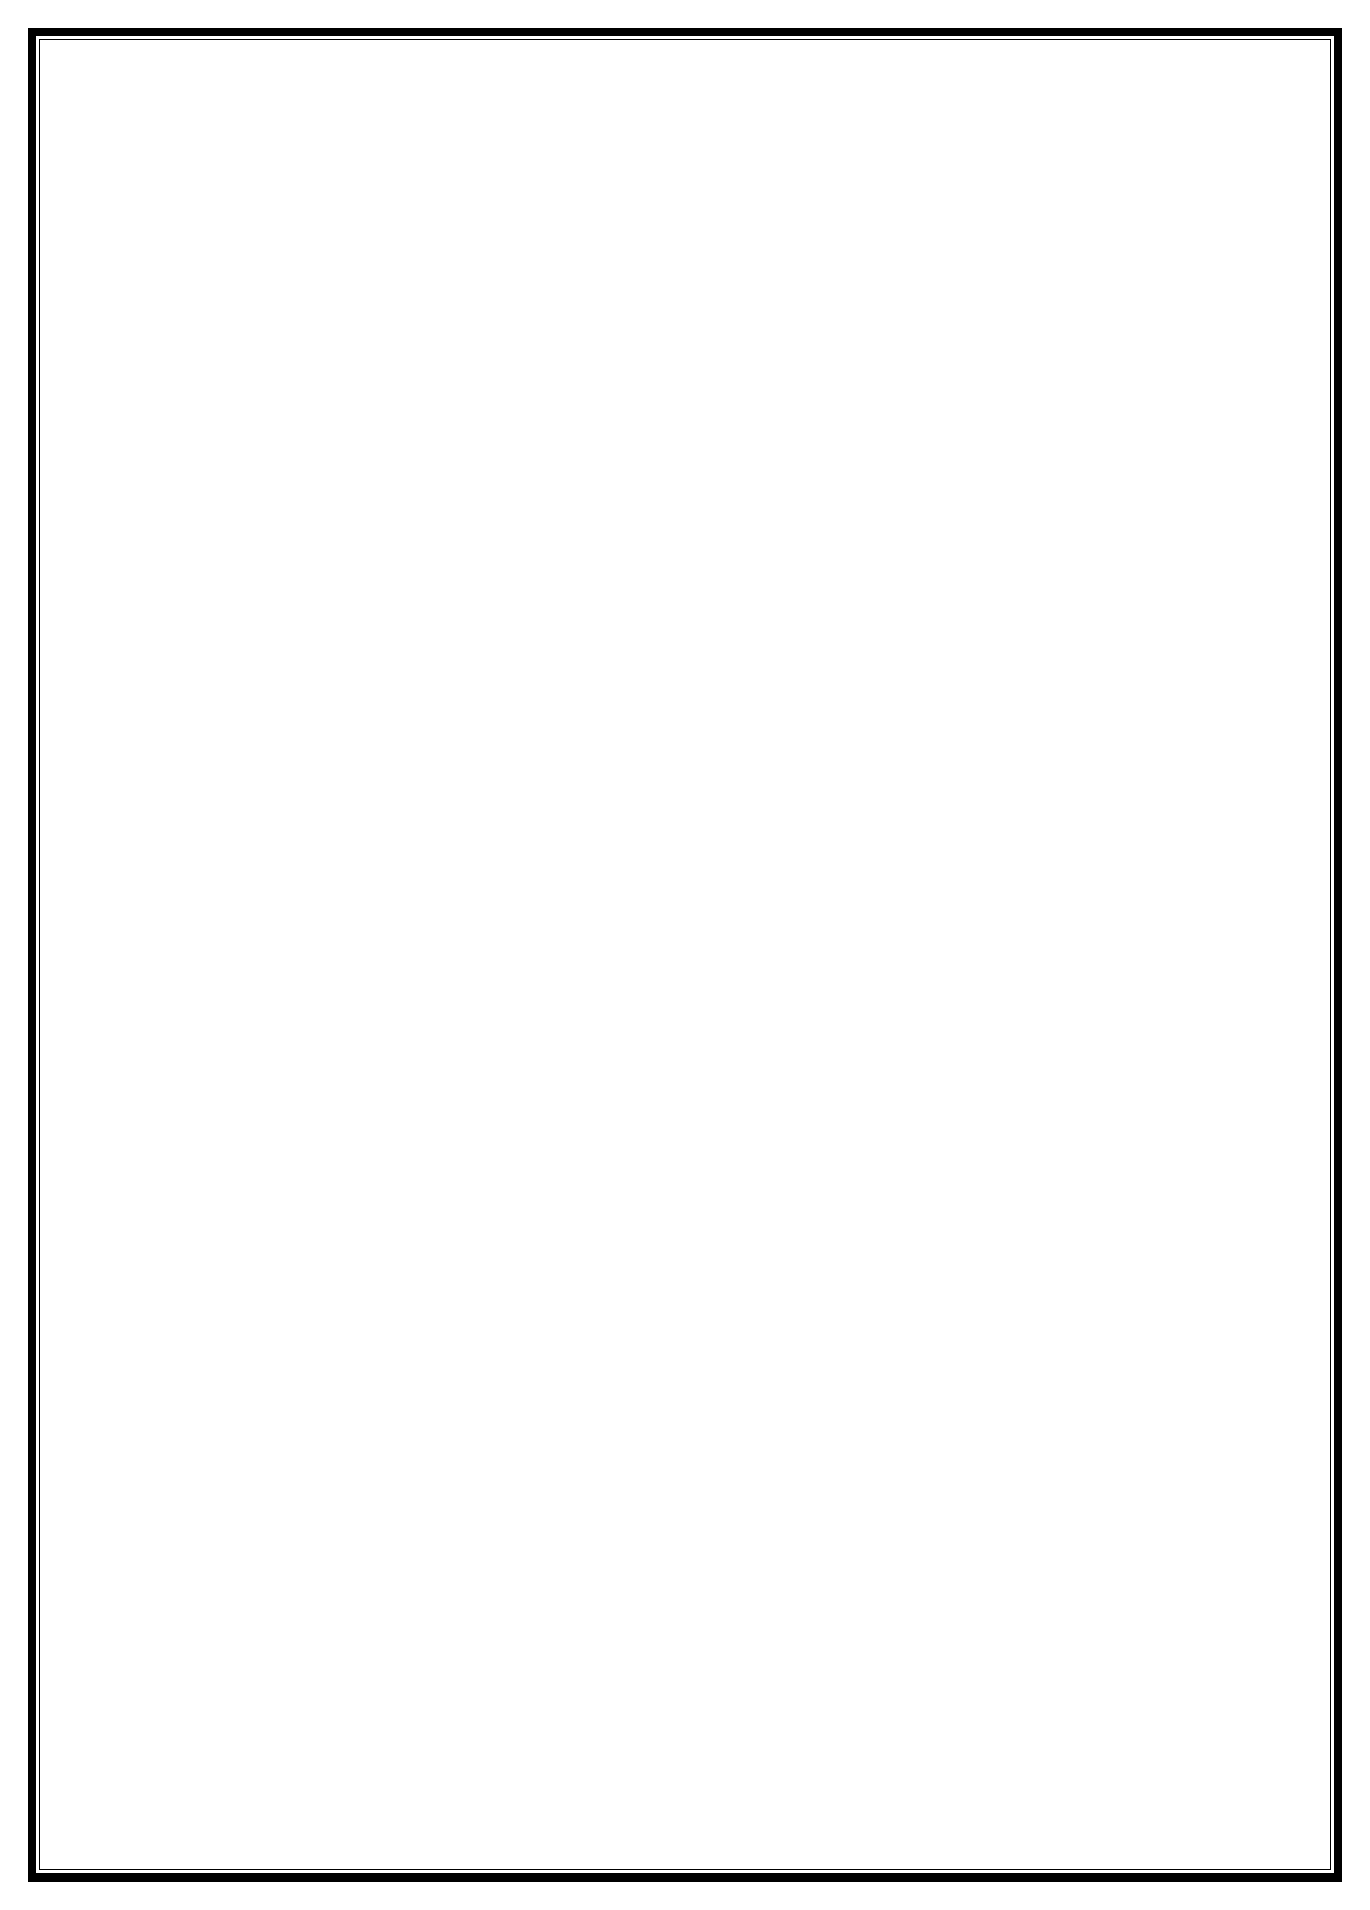
\begin{tikzpicture}
    \draw[line width=3pt] ($ (current page.north west) + (3.0cm,-2.0cm) $) rectangle ($ (current page.south east) + (-2.0cm,2.5cm) $);
    \draw[line width=0.5pt] ($ (current page.north west) + (3.1cm,-2.1cm) $) rectangle ($ (current page.south east) + (-2.1cm,2.6cm) $);
    \end{tikzpicture}
\end{titlepage}
\end{document}
